\chapter{Eksperymenty i analiza}\label{chap:experiments}

\section{Środowisko obliczeniowe}

Badania eksperymentalne przeprowadzono na komputerze wyposażonym w procesor Intel Core i5-14600KF (12 rdzeni, taktowanie 3,49 GHz) oraz 16 GB pamięci RAM. Jako system operacyjny wykorzystano Ubuntu 24.04 LTS uruchomiony w środowisku WSL2. Wszystkie algorytmy zaimplementowano w języku Python 3.13 z użyciem bibliotek NumPy do operacji numerycznych, NetworkX do pracy z grafami oraz PuLP jako interfejs do solverów programowania liniowego. Podczas pomiarów wydajności mierzono wyłącznie czas wykonania algorytmów, pomijając operacje wejścia-wyjścia i przygotowania struktur danych.

\section{Metodologia eksperymentów}

\subsection{Protokół badawczy}

W celu zapewnienia kontrolowanych warunków eksperymentalnych, każdy algorytm uruchamiano w oddzielnym procesie systemowym z ustalonym limitem czasu wykonania wynoszącym 60 sekund. Przekroczenie tego limitu skutkowało oznaczeniem wyniku jako \texttt{timeout} i wykluczeniem go z analizy.

Schemat powtórzeń eksperymentalnych przedstawiał się następująco:

\begin{itemize}
  \item \textbf{Grafy syntetyczne}: 3 próbki na rozmiar, 2 powtórzenia na próbkę
  \item \textbf{Grafy rzeczywiste}: 2 powtórzenia na graf ego
\end{itemize}

\begin{table}[H]
  \caption{Zestaw algorytmów analizowanych w eksperymentach.}
  \label{tab:algorithms}
  \centering
  \begin{tabular}{lll}
    \toprule
    \textbf{Algorytm}              & \textbf{Klasa}              & \textbf{Charakterystyka}                         \\
    \midrule
    metoda ILP                     & Dokładny (ILP)              & Optymalne rozwiązania dla małych instancji       \\
    heurystyka zbioru dominującego & Heurystyka deterministyczna & Aproksymacja zbioru dominującego                 \\
    algorytm zachłanny             & Heurystyka zachłanna        & Lokalny wybór właściciela o największym pokryciu \\
    algorytm losowy                & Heurystyka losowa           & Losowy przydział licencji w ramach ograniczeń    \\
    algorytm genetyczny            & Metaheurystyka              & Selekcja turniejowa, krzyżowanie jednopunktowe   \\
    symulowane wyżarzanie          & Metaheurystyka              & Eksploracja stanu z harmonogramem chłodzenia     \\
    przeszukiwanie tabu            & Metaheurystyka              & Przeszukiwanie lokalne z listą tabu i aspiracją  \\
    algorytm mrówkowy              & Metaheurystyka              & Konstrukcja rozwiązań sterowana feromonami       \\
    \bottomrule
  \end{tabular}
\end{table}

W procesie analizy uwzględniano jedynie te obserwacje, które zostały oznaczone flagą \texttt{valid=True} oraz nie nosiły statusu \texttt{timeout} ani \texttt{error}. Tak przygotowane dane poddano agregacji statystycznej z wykorzystaniem średniej arytmetycznej wraz z obliczeniem odchylenia standardowego.

\subsection{Analiza statystycznej istotności wyników}

Aby ocenić, czy zaobserwowane różnice w wydajności algorytmów mają charakter systematyczny czy przypadkowy, przeprowadzono szczegółową analizę statystyczną. Obliczono odchylenia standardowe oraz 95-procentowe przedziały ufności dla średnich wartości kosztów i czasów wykonania. Dodatkowo zastosowano nieparametryczne testy statystyczne do porównania wydajności poszczególnych metod.

\paragraph{Odchylenia standardowe i przedziały ufności}

Dla zbioru syntetycznego każda metoda miała co najmniej 100 obserwacji, co pozwoliło wyznaczyć wiarygodne 95-procentowe przedziały ufności:

\begin{table}[H]
  \caption{Średnie koszty i czasy wykonania (ze standardowym odchyleniem) dla wybranych algorytmów na grafach syntetycznych.}
  \label{tab:synthetic_alg_performance}
  \centering
  \begin{tabular}{lcc}
    \toprule
    \textbf{Algorytm}              & \textbf{Średni koszt $\pm$ std} & \textbf{Czas [ms] $\pm$ std} \\
    \midrule
    metoda ILP                     & 1033 $\pm$ 269                  & 2492 $\pm$ 851               \\
    algorytm mrówkowy              & 1169 $\pm$ 149                  & 5124 $\pm$ 1232              \\
    przeszukiwanie tabu            & 1648 $\pm$ 259                  & 3298 $\pm$ 683               \\
    heurystyka zbioru dominującego & 1678 $\pm$ 251                  & 16,7 $\pm$ 5,1               \\
    algorytm zachłanny             & 1706 $\pm$ 256                  & 0,96 $\pm$ 0,19              \\
    \bottomrule
  \end{tabular}
\end{table}

Analiza przedziałów ufności wykazuje brak ich nakładania się między metodą ILP a pozostałymi algorytmami, co stanowi silny dowód na systematyczną przewagę jakościową tej metody. Podobnie, różnice w wydajności między poszczególnymi metaheurystykami przewyższają szerokość ich przedziałów ufności, co świadczy o istotności statystycznej zaobserwowanych różnic.

Dla grafów ego z serwisu Facebook zastosowano mniejszą liczbę powtórzeń (12--20), co rezultuje szerszymi przedziałami ufności. Na przykład algorytm mrówkowy osiągnął średni koszt 1155 ± 432 przy czasie wykonania 14~055 ms ± 8685 ms, podczas gdy przeszukiwanie tabu uzyskało średni koszt 1463 ± 679 przy czasie 17~777 ms ± 10~432 ms. W przypadku metody ILP, tylko jedna instancja została ukończona w zadanym limicie czasu 60 sekund, natomiast pozostałe zakończyły się przekroczeniem limitu. Z tego względu metoda ILP nie jest uwzględniana w dalszej analizie porównawczej dla grafów ego.

\paragraph{Weryfikacja hipotez statystycznych}

Dla zbioru grafów syntetycznych zastosowano test Friedmana \cite{friedman1937}, analizując rangi kosztów i czasów wykonania z traktowaniem każdej instancji grafu jako osobnego bloku eksperymentalnego. Uzyskane wyniki wykazują istotność statystyczną na poziomie $p < 0{,}001$, co pozwala odrzucić hipotezę zerową o braku różnic między algorytmami. Przeprowadzony następnie test post-hoc Nemenyiego \cite{nemenyi1963}, zgodnie z rekomendacjami przeglądowymi dla porównań wielu algorytmów \cite{demsar2006}, ujawnił następujące zależności:

\begin{itemize}
  \item \textbf{metoda ILP} różni się istotnie od wszystkich pozostałych metod
  \item \textbf{algorytm mrówkowy} różni się od wszystkich heurystyk i większości metaheurystyk, lecz mniej wyraźnie od przeszukiwania tabu
  \item \textbf{algorytm zachłanny} i \textbf{algorytm losowy} tworzą grupę najsłabszych wyników i różnią się istotnie od wszystkich pozostałych
\end{itemize}

Ze względu na ograniczoną liczbę obserwacji dla grafów ego, zastosowane testy charakteryzują się mniejszą mocą statystyczną. Niemniej jednak wstępne wyniki sugerują zachowanie podobnej hierarchii wydajności algorytmów.

\section{Ograniczenia badań}

\subsection{Ograniczenia metodologiczne}

Przeprowadzone eksperymenty charakteryzują się kilkoma istotnymi ograniczeniami metodologicznymi. Po pierwsze, badania obejmowały jedynie trzy klasy grafów syntetycznych oraz 10 rzeczywistych sieci ego, co stanowi reprezentatywną, lecz ograniczoną próbę możliwych struktur sieciowych. Pominięto inne istotne rodzaje grafów, takie jak drzewa, struktury z hiper-krawędziami, grafy skierowane czy sieci wielowarstwowe, przez co uzyskane wyniki mogą nie być w pełni reprezentatywne dla grafów o zasadniczo odmiennej topologii.

Po drugie, metodę ILP testowano wyłącznie na grafach małej wielkości, co uniemożliwia ocenę jej efektywności na sieciach większych rozmiarów. Jednocześnie algorytmy metaheurystyczne dla instancji o wielkości $n > 1000$ mogą wymagać dodatkowego dostrojenia parametrów w celu osiągnięcia optymalnej wydajności.

\subsection{Ograniczenia techniczne i pomiarowe}

Istotne ograniczenia wynikają również z aspektów technicznych eksperymentów. Zarówno proces generowania grafów syntetycznych, jak i działanie algorytmów metaheurystycznych opiera się na sekwencjach pseudolosowych. Mimo zastosowania deterministycznych seedów, pewien poziom wariancji wyników pozostaje nieunikniony, co może wpływać na powtarzalność rezultatów.

Pomiary czasu wykonania obejmują overhead systemowy, który może różnić się między platformami sprzętowymi. Szczególnie dla algorytmów długotrwałych (algorytm mrówkowy, przeszukiwanie tabu) naturalne fluktuacje czasowe mogą być statystycznie istotne, co należy uwzględnić przy interpretacji wyników porównawczych.

Wymienione ograniczenia wymagają ostrożnej interpretacji uzyskanych rezultatów. Przedstawione wyniki należy traktować jako wskazówki metodologiczne dotyczące wyboru algorytmu w analogicznych warunkach eksperymentalnych. Należy mieć na uwadze, że względna hierarchia wydajności algorytmów mogłaby ulec zmianie w przypadku zastosowania innych parametrów metaheurystyk lub wydłużenia limitów czasowych. Niemniej jednak obserwowana spójność wyników między różnymi typami struktur grafowych dostarcza solidnej podstawy dla formułowania praktycznych rekomendacji.

\section{Charakterystyka zbiorów danych}

Materiał badawczy składał się z dwóch niezależnych kolekcji danych eksperymentalnych:

\begin{itemize}
  \item \textbf{Syntetyczne grafy} -- trójelementowy zestaw generatorów (\emph{random}, \emph{small\_world}, \emph{scale\_free}) tworzył sieci o liczbie węzłów od 20 do 200 (co 20) oraz większe rozmiary 300, 400, 600, 800, 1000. Dla każdej kombinacji typu grafu i rozmiaru generowano trzy próbki, a następnie dla każdej z nich uruchamiano osiem algorytmów (\textbf{metoda ILP}, \textbf{algorytm zachłanny}, \textbf{algorytm losowy}, \textbf{heurystyka zbioru dominującego}, \textbf{algorytm mrówkowy}, \textbf{symulowane wyżarzanie}, \textbf{przeszukiwanie tabu}, \textbf{algorytm genetyczny}) w dwóch powtórzeniach. Badano dwie główne konfiguracje licencji: \emph{duolingo\_super} i \emph{roman\_domination}. Pomiar obejmował koszt całkowity \texttt{total\_cost}, czas wykonania \texttt{time\_ms} oraz poprawność rozwiązania \texttt{valid}.

  \item \textbf{Grafy facebook ego} -- dziesięć grafów ego pobranych z bazy SNAP (rozmiary 53--1035 węzłów) reprezentowało sieci rzeczywiste. Uruchomiono te same algorytmy i konfiguracje licencji, odnotowując te same metryki co dla grafów syntetycznych.
\end{itemize}

Dla obu kolekcji danych zastosowano jednolitą procedurę filtracji, wykluczając z analizy wyniki oznaczone statusami \texttt{timeout} lub \texttt{error}, a także obserwacje niespełniające warunków poprawności (\texttt{valid=False}).

\section{Analiza wyników dla grafów syntetycznych}

Po zastosowaniu procedur filtracji na zbiorze grafów syntetycznych uzyskano 1972 prawidłowych uruchomień algorytmów, które dotyczyły konfiguracji licencyjnej \emph{duolingo\_super}.

\subsection{Analiza rozkładów kosztów i czasów wykonania}

Rysunek \ref{fig:synthetic_cost_boxplot} przedstawia rozkład całkowitych kosztów \texttt{total\_cost} w przekroju badanych algorytmów. Wyniki wyraźnie wskazują na dominację \textbf{metody ILP}, która osiąga najniższe wartości kosztowe, aczkolwiek jej zastosowanie ogranicza się do grafów o niewielkich rozmiarach. W grupie algorytmów metaheurystycznych najlepszą jakość rozwiązań demonstruje \textbf{algorytm mrówkowy}, podczas gdy \textbf{algorytm zachłanny} charakteryzuje się znacznie wyższymi kosztami. Dla porównania, \textbf{algorytm losowy} służący jako baseline potwierdza skuteczność metod heurystycznych -- wszystkie badane algorytmy przewyższają losowe przydzielanie licencji.

\begin{figure}[H]
  \centering
  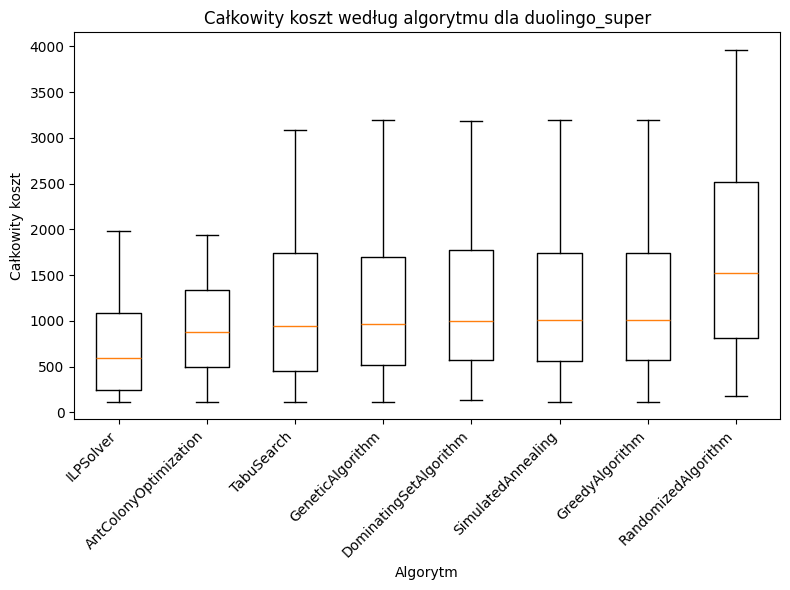
\includegraphics[width=0.7\linewidth]{assets/figures/synthetic_cost_boxplot.png}
  \caption{Całkowity koszt według algorytmu dla konfiguracji duolingo\_super.}
  \label{fig:synthetic_cost_boxplot}
\end{figure}

Analiza czasów wykonania, przedstawiona na rysunku \ref{fig:synthetic_time_boxplot} w skali logarytmicznej, ujawnia wyraźne zróżnicowanie wydajnościowe algorytmów. Metody zachłanne oraz losowe zdecydowanie dominują pod względem szybkości. Warto zauważyć, że średni czas działania \textbf{algorytmu mrówkowego} i \textbf{przeszukiwania tabu} bywa wyższy niż \textbf{metody ILP} ze względu na limit 60 s. Czas ILP rósł szybciej wraz z liczbą węzłów, przez co wiele uruchomień zakończyło się statusem \texttt{timeout} i zostało wykluczonych z analizy. Średnia liczona jest więc głównie dla mniejszych instancji. Z kolei \textbf{przeszukiwanie tabu} i \textbf{algorytm mrówkowy} zwiększały czas wolniej, częściej kończąc tuż poniżej limitu, co powoduje, że ich średni czas oscyluje bliżej granicy 60 s i finalnie przewyższa średni czas ILP przy większej liczbie próbek.

\begin{figure}[H]
  \centering
  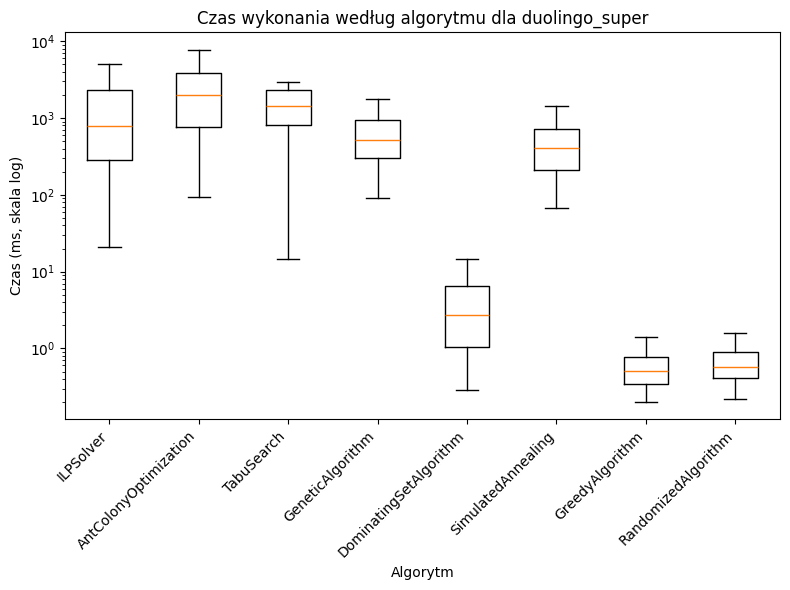
\includegraphics[width=0.7\linewidth]{assets/figures/synthetic_time_boxplot.png}
  \caption{Czas wykonania według algorytmu dla konfiguracji duolingo\_super.}
  \label{fig:synthetic_time_boxplot}
\end{figure}

\subsection{Zależność wydajności od wielkości grafu}

Analiza wpływu liczby węzłów na średni koszt rozwiązań, przedstawiona na rysunku \ref{fig:synthetic_cost_vs_nodes}, wykazuje tendencję wzrostową kosztów wraz ze zwiększaniem się rozmiaru grafu. \textbf{metoda ILP} utrzymuje pozycję lidera pod względem jakości rozwiązań dla grafów o wielkości do około $n \approx 200$ węzłów. \textbf{algorytm mrówkowy} plasuje się na drugiej pozycji, jednak dla grafów większych rozmiarów obserwuje się stopniowy wzrost generowanych kosztów. Pozostałe algorytmy metaheurystyczne tworzą względnie zwartą grupę wyników. Co istotne, \textbf{algorytm zachłanny} osiąga koszty jedynie nieznacznie wyższe od metaheurystyk i pozostaje jakościowo konkurencyjny w całym badanym zakresie rozmiarów. Wyraźnie gorsze rezultaty notuje jedynie \textbf{algorytm losowy}, którego koszt utrzymuje się na istotnie wyższym poziomie niezależnie od liczby węzłów.

\begin{figure}[H]
  \centering
  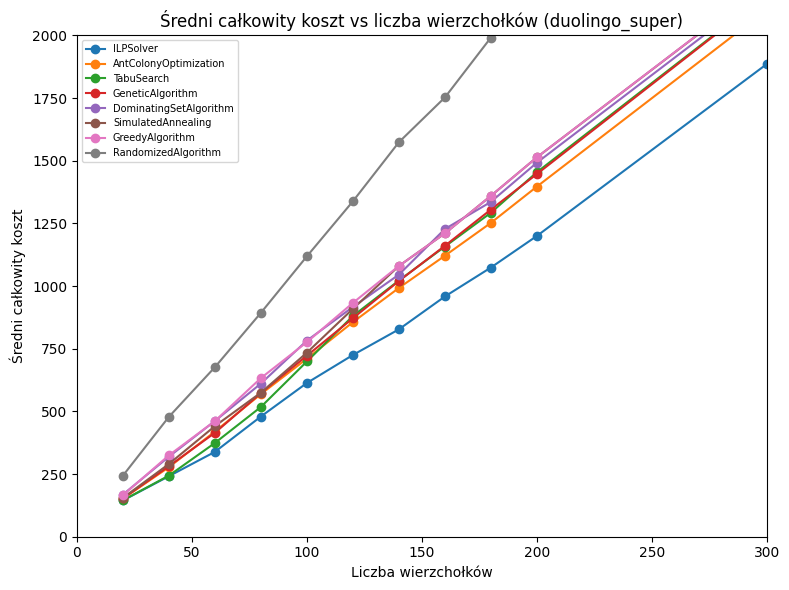
\includegraphics[width=0.7\linewidth]{assets/figures/synthetic_cost_vs_nodes.png}
  \caption{Średni całkowity koszt vs liczba węzłów.}
  \label{fig:synthetic_cost_vs_nodes}
\end{figure}

Analogicznie, czasy obliczeń pokazane na rysunku \ref{fig:synthetic_time_vs_nodes} na osi logarytmicznej rosną wolno (w przybliżeniu logarytmicznie) wraz z liczbą węzłów. \textbf{algorytm zachłanny} i \textbf{algorytm losowy} pozostają niemal niezależne od rozmiaru, a \textbf{heurystyka zbioru dominującego} rośnie umiarkowanie. Wysoki koszt czasowy \textbf{algorytmu mrówkowego} wynika w dużej mierze z braku równoległości w implementacji. Algorytm działa w jednym wątku i nie wykorzystuje niezależnej ewaluacji mrówek. Równoleglenie (wielowątkowość/multiprocessing lub wektoryzacja) powinno istotnie obniżyć czas i spłaszczyć krzywą.

\begin{figure}[H]
  \centering
  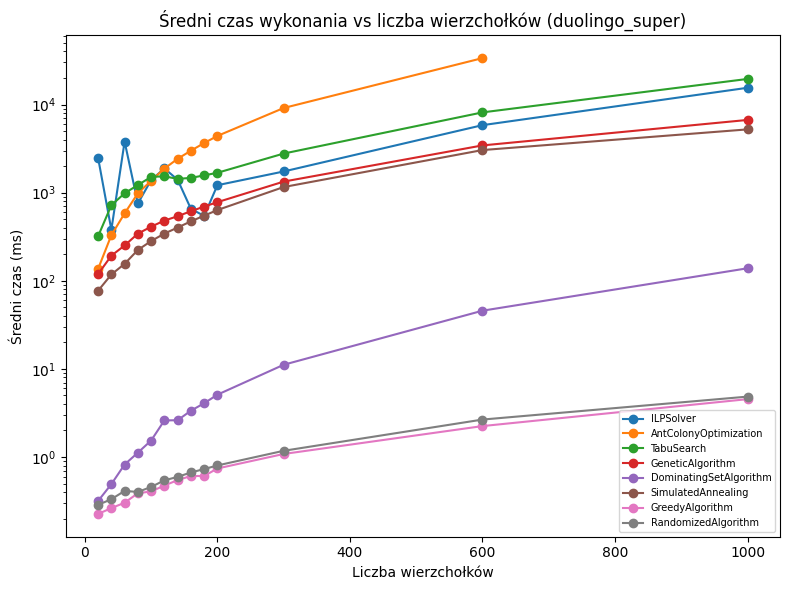
\includegraphics[width=0.7\linewidth]{assets/figures/synthetic_time_vs_nodes.png}
  \caption{Średni czas wykonania vs liczba węzłów.}
  \label{fig:synthetic_time_vs_nodes}
\end{figure}

\subsection{Kompromis koszt--czas}

Wykres Pareto (rys. \ref{fig:synthetic_pareto}) ilustruje zależność między kosztem a czasem. Najkorzystniejsze punkty należą do \textbf{metody ILP} i \textbf{algorytmu mrówkowego}, lecz czas drugiego z nich jest wielokrotnie większy. \textbf{przeszukiwanie tabu} i \textbf{algorytm genetyczny} zapewniają przyzwoite koszty przy umiarkowanych czasach, natomiast algorytm zachłanny i algorytm losowy pozostają najszybsze.

\begin{figure}[H]
  \centering
  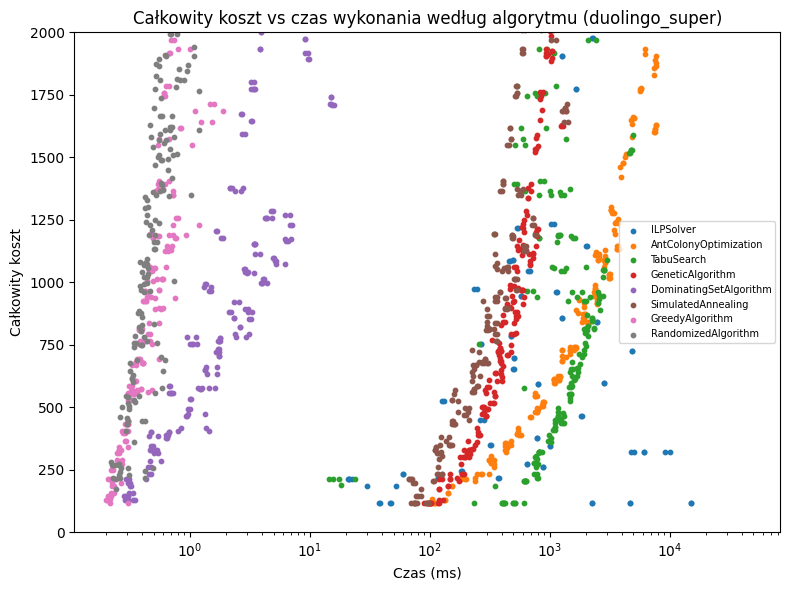
\includegraphics[width=0.7\linewidth]{assets/figures/synthetic_pareto.png}
  \caption{Całkowity koszt vs czas wykonania.}
  \label{fig:synthetic_pareto}
\end{figure}

\subsection{Koszt na węzeł i rozrzut czasów}

Rozkład kosztu w przeliczeniu na węzeł (rys. \ref{fig:synthetic_cost_per_node}) potwierdza przewagę metody ILP i algorytmu mrówkowego, a rozrzut czasów w zależności od liczby węzłów (rys. \ref{fig:synthetic_time_scatter}) pokazuje silną zależność czasową dla metaheurystyk (współczynnik korelacji z liczbą węzłów sięga 0,90) i niewielki wpływ gęstości grafu (korelacje ujemne --0,05 do --0,30).

\begin{figure}[H]
  \centering
  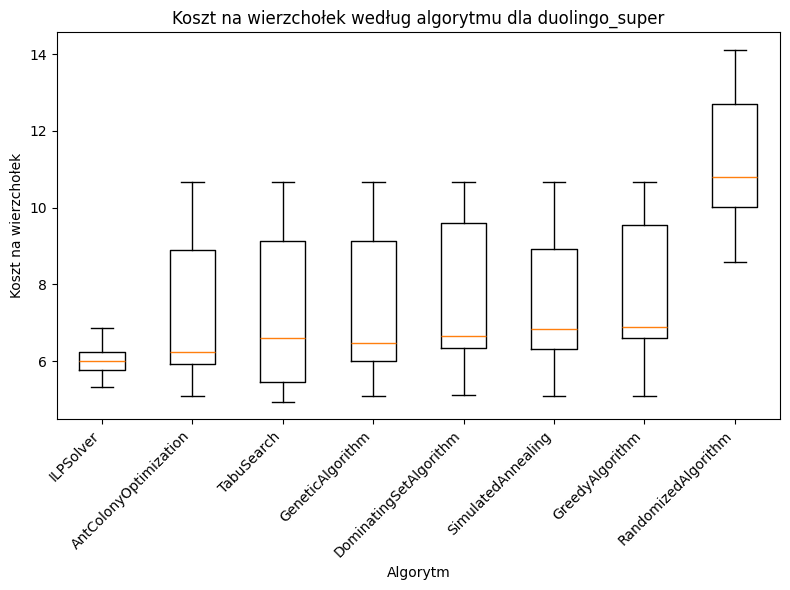
\includegraphics[width=0.7\linewidth]{assets/figures/synthetic_cost_per_node.png}
  \caption{Koszt na węzeł według algorytmu.}
  \label{fig:synthetic_cost_per_node}
\end{figure}

\begin{figure}[H]
  \centering
  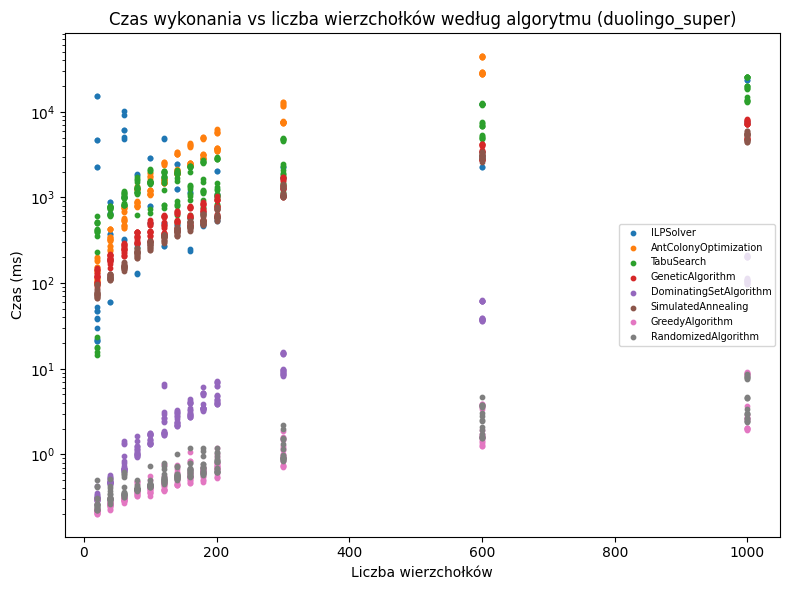
\includegraphics[width=0.7\linewidth]{assets/figures/synthetic_time_scatter.png}
  \caption{Czas wykonania vs liczba węzłów.}
  \label{fig:synthetic_time_scatter}
\end{figure}

\section{Analiza grafów facebook ego}

Eksperymenty na sieciach ego objęły 10 grafów o wielkości 53--1035 węzłów. Z 320 uruchomień zachowano 288 poprawnych obserwacji. Ze względu na to, że \textbf{metoda ILP} ukończyła obliczenia w czasie jedynie dla jednej próbki ego (pozostałe uruchomienia zakończyły się \texttt{timeout}), została ona \emph{pominięta w dalszej analizie porównawczej} dla tego zbioru. Wnioski w tym podrozdziale dotyczą zatem wyłącznie metod heurystycznych i metaheurystycznych.

\subsection{Rozkład kosztów i czasów}

Rysunek \ref{fig:facebook_cost_boxplot} przedstawia koszty dla \emph{duolingo\_super} na grafach facebookowych. Wśród metod przybliżonych \textbf{algorytm mrówkowy} i \textbf{przeszukiwanie tabu} należą do najlepszych jakościowo, przy czym pozostałe algorytmy osiągają zbliżone koszty. Co istotne, \textbf{algorytm zachłanny} uzyskuje koszty porównywalne z grupą metaheurystyk, natomiast \textbf{algorytm losowy} konsekwentnie wypada znacznie gorzej i pełni rolę baseline.

\begin{figure}[H]
  \centering
  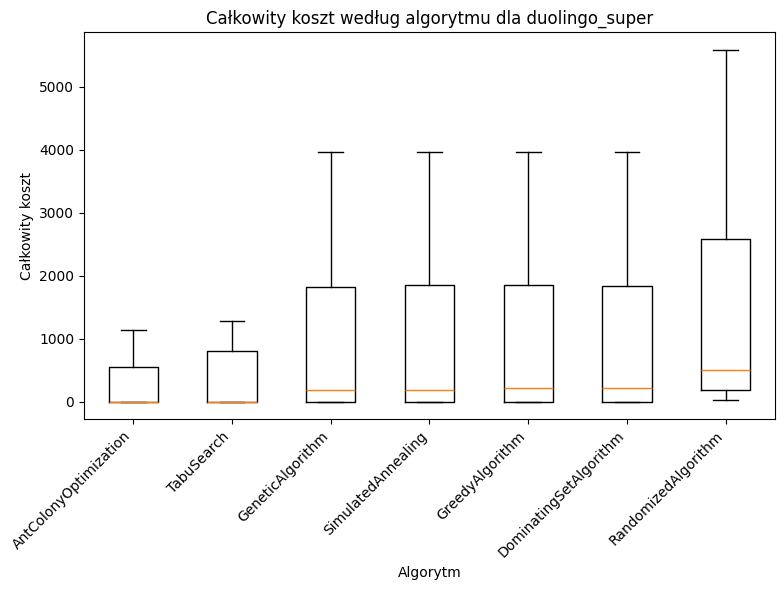
\includegraphics[width=0.7\linewidth]{assets/figures/facebook_cost_boxplot.png}
  \caption{Całkowity koszt według algorytmu dla konfiguracji duolingo\_super dla grafu ego facebook.}
  \label{fig:facebook_cost_boxplot}
\end{figure}

Czas działania (rys. \ref{fig:facebook_time_boxplot}) pokazuje, że \emph{na grafach ego najlepsze czasy osiągają} \textbf{algorytm mrówkowy} oraz \textbf{przeszukiwanie tabu} (rzędu 8--10 s), podczas gdy pozostałe metody wypadają porównywalnie lub wolniej.

\begin{figure}[H]
  \centering
  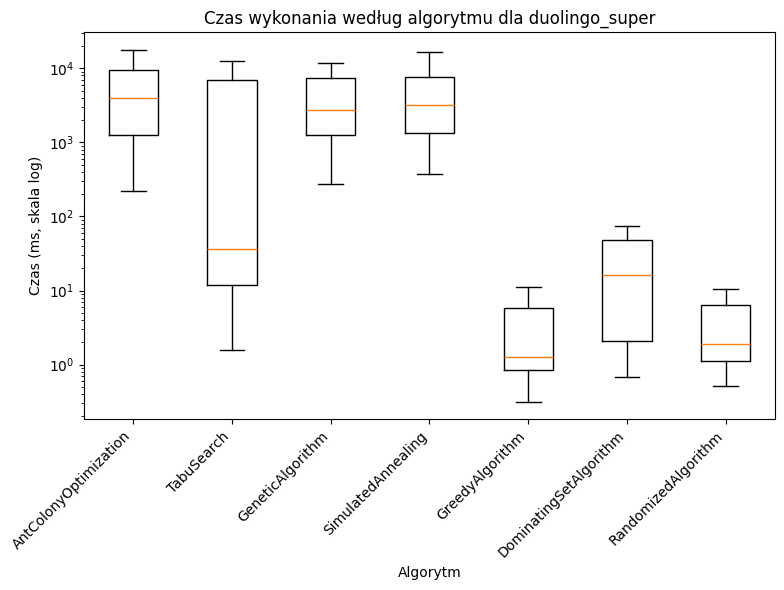
\includegraphics[width=0.7\linewidth]{assets/figures/facebook_time_boxplot.png}
  \caption{Czas wykonania według algorytmu dla konfiguracji duolingo\_super dla grafu ego facebook.}
  \label{fig:facebook_time_boxplot}
\end{figure}

\subsection{Zależność od liczby węzłów}

Średnie koszty dla grafów ego (rys. \ref{fig:facebook_cost_vs_nodes}) rosną wraz z rozmiarem. \textbf{przeszukiwanie tabu} wyraźnie osiąga niższe koszty od pozostałych metod, które grupują się blisko siebie pod względem jakości. Wyjątek stanowi \textbf{algorytm losowy}, którego koszt jest istotnie wyższy w całym zakresie rozmiarów.

\begin{figure}[H]
  \centering
  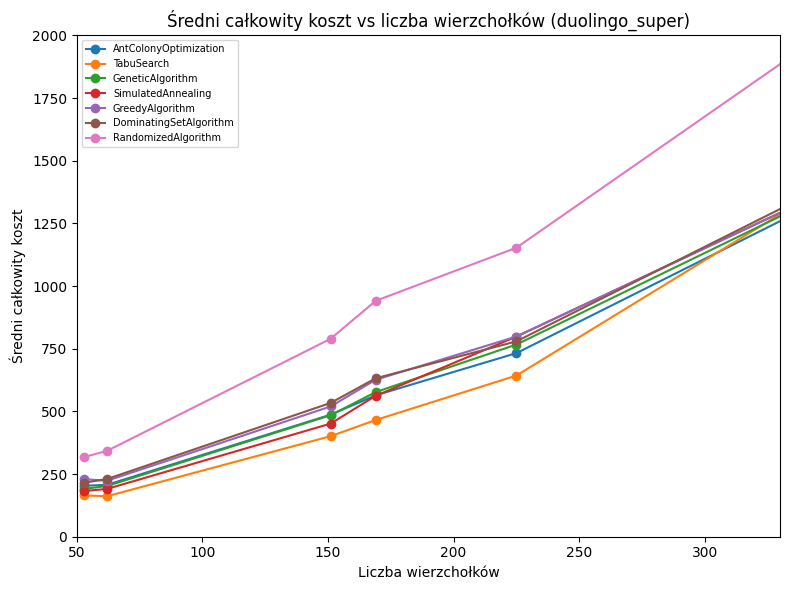
\includegraphics[width=0.7\linewidth]{assets/figures/facebook_cost_vs_nodes.png}
  \caption{Średni całkowity koszt vs liczba węzłów dla grafu ego facebook.}
  \label{fig:facebook_cost_vs_nodes}
\end{figure}

Wykres czasów (rys. \ref{fig:facebook_time_vs_nodes}) ukazuje, że \textbf{algorytm mrówkowy} i \textbf{przeszukiwanie tabu} utrzymują najlepsze czasy w przekroju rozmiarów, podczas gdy pozostałe metody wykazują porównywalny lub wyższy czas wykonania.

\begin{figure}[H]
  \centering
  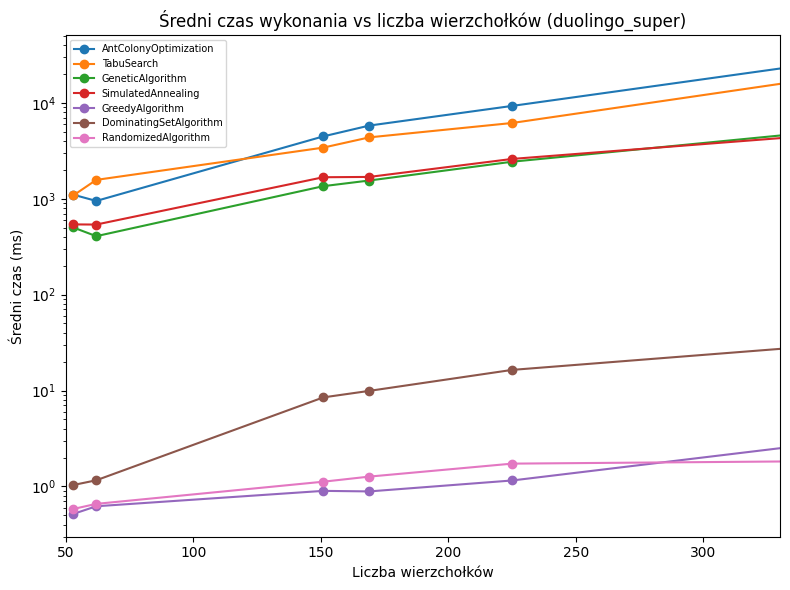
\includegraphics[width=0.7\linewidth]{assets/figures/facebook_time_vs_nodes.png}
  \caption{Średni czas wykonania vs liczba węzłów dla grafu ego facebook.}
  \label{fig:facebook_time_vs_nodes}
\end{figure}

\subsection{Kompromis koszt--czas i koszt na węzeł}

Wykres Pareto (rys. \ref{fig:facebook_pareto}) dla grafów ego pokazuje mniejszą liczbę punktów: \textbf{algorytm mrówkowy} i \textbf{przeszukiwanie tabu} tworzą front optymalny, podczas gdy algorytm genetyczny i symulowane wyżarzanie dostarczają kompromisy. Algorytm zachłanny oraz algorytm losowy są zdominowane kosztowo i/lub czasowo w tym zbiorze.

\begin{figure}[H]
  \centering
  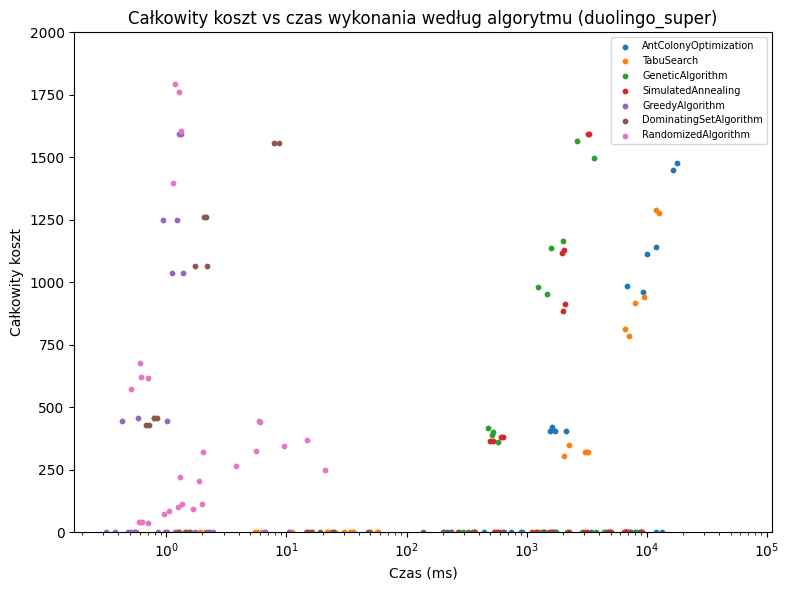
\includegraphics[width=0.7\linewidth]{assets/figures/facebook_pareto.png}
  \caption{Całkowity koszt vs czas wykonania dla grafu ego facebook.}
  \label{fig:facebook_pareto}
\end{figure}

Rozkład kosztu na węzeł (rys. \ref{fig:facebook_cost_per_node}) pokazuje, że \textbf{jedynie przeszukiwanie tabu wyraźnie odznacza się najniższym kosztem per wierzchołek}. Może to sugerować, że ten konkretny algorytm lepiej wykorzystuje właściwości rzeczywistych sieci ego niż pozostałe metody, które na syntetycznych grafach osiągały wyniki zbliżone do \textbf{algorytmu zachłannego}.

\begin{figure}[H]
  \centering
  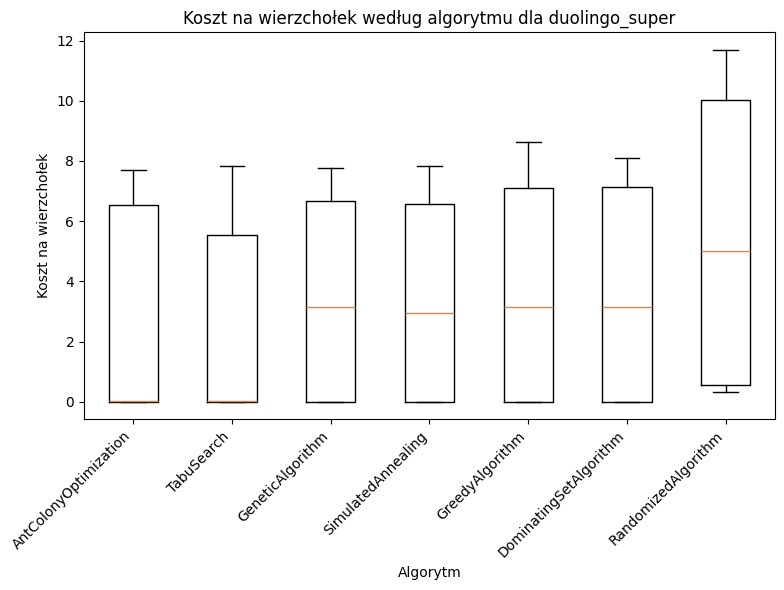
\includegraphics[width=0.7\linewidth]{assets/figures/facebook_cost_per_node.png}
  \caption{Koszt na węzeł według algorytmu dla grafu ego facebook.}
  \label{fig:facebook_cost_per_node}
\end{figure}

Rozrzut czasów w zależności od liczby węzłów (rys. \ref{fig:facebook_time_scatter}) pokazuje, że metaheurystyki wykazują silniejszą zależność od rozmiaru grafu (korelacje $\sim$0,9) niż heurystyki.

\begin{figure}[H]
  \centering
  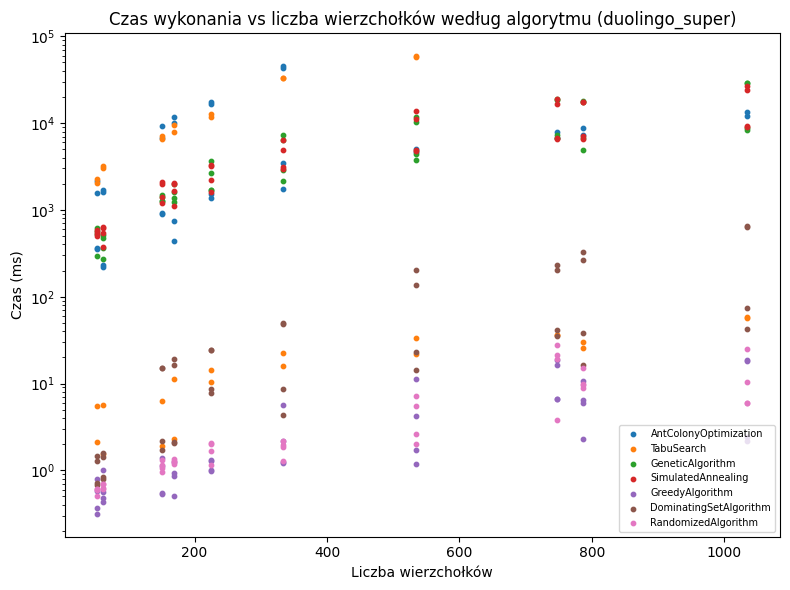
\includegraphics[width=0.7\linewidth]{assets/figures/facebook_time_scatter.png}
  \caption{Czas wykonania vs liczba węzłów dla grafu ego facebook.}
  \label{fig:facebook_time_scatter}
\end{figure}

\section{Analiza i wnioski}

Przeprowadzona analiza porównawcza grafów syntetycznych oraz rzeczywistych sieci ego z Facebooka ujawnia spójne wzorce, ale także istotne różnice wynikające ze struktury danych. W syntetykach (ER/WS/BA) obserwujemy klasyczną hierarchię: ILP wyznacza dolną granicę jakości na małych instancjach, \textbf{algorytm mrówkowy} i \textbf{przeszukiwanie tabu} dostarczają najlepszych kosztów wśród metod przybliżonych, a \textbf{algorytm zachłanny} pozostaje szybkim punktem odniesienia kosztem nieco wyższych, lecz wciąż zadowalających, wartości celu. \textbf{algorytm losowy} pełni rolę baseline i jest konsekwentnie najsłabszy jakościowo.

Na realnych sieciach ego, gdzie ILP został pominięty z uwagi na zbyt małą liczbę ukończonych w czasie instancji, obraz jest odmienny w dwóch kluczowych aspektach: (i) \textbf{przeszukiwanie tabu} osiąga \emph{najniższe koszty} i wyraźnie odcina się od pozostałych metod, które grupują się blisko siebie (z wyjątkiem \textbf{algorytmu losowego}, znacząco gorszego); (ii) \textbf{algorytm mrówkowy} i \textbf{przeszukiwanie tabu} osiągają \emph{najlepsze czasy wykonania} w przekroju rozmiarów ego, co sugeruje ich lepsze dopasowanie do właściwości rzeczywistych struktur. Dodatkowo w metryce kosztu na węzeł jedynie \textbf{przeszukiwanie tabu} wyraźnie się wyróżnia, podczas gdy na grafach syntetycznych jego wyniki były bliższe \textbf{algorytmu zachłannego}. To wskazuje, że tabu może lepiej wykorzystywać lokalne wzorce klastrowania i stopnie hubów obecne w ego-sieciach.

Z perspektywy skalowalności, czasy metod metaheurystycznych rosną z rozmiarem, jednak na realnych danych przewagi algorytmu mrówkowego i przeszukiwania tabu w czasie oraz przewaga przeszukiwania tabu w koszcie utrzymują się w całym badanym zakresie. W efekcie w analizie Pareto dla ego to \textbf{algorytm mrówkowy} i \textbf{przeszukiwanie tabu} budują front niezdominowanych rozwiązań, podczas gdy algorytm genetyczny/symulowane wyżarzanie pozostają kompromisami, a algorytm zachłanny/algorytm losowy są zdominowane.

Praktyczne implikacje są następujące: (1) dla grafów syntetycznych i małych instancji warto korzystać z ILP jako punktu odniesienia jakości, a w większej skali wybierać \textbf{algorytm mrówkowy/przeszukiwanie tabu} dla jakości lub \textbf{algorytm zachłanny} dla szybkości; (2) dla rzeczywistych sieci ego rekomendowanym wyborem jest \textbf{przeszukiwanie tabu} jako metoda zapewniająca \emph{najniższy koszt (również per węzeł)} przy jednocześnie konkurencyjnych czasach, a \textbf{algorytm mrówkowy} jako alternatywa, gdy zależy nam na podobnym profilu czasowym i wysokiej jakości; (3) \textbf{algorytm zachłanny} pozostaje użyteczny jako bardzo szybka inicjalizacja (warm start) i w świetle przeprowadzonych testów nie jest wyraźnie gorszy od metaheurystyk w większości przetestowanych ustawień. Różnice jakości mogą się uwidocznić przy \emph{dużo większych grafach}, \emph{lepszym dostrojeniu hiperparametrów} oraz przy \emph{dłuższych budżetach czasu} (znosząc twardy limit 60 s), nadal pozostając wyraźnie szybszym rozwiązaniem niż ILP. Jeśli niewielka poprawa kosztu nie jest kluczowa biznesowo, prosty algorytm zachłanny może być wystarczający dla wielu zastosowań; (4) \textbf{algorytm losowy} należy traktować wyłącznie jako baseline.
